\begin{frame}{Support Vector Classifier}
\begin{columns}
  \begin{column}{0.5\textwidth}
    \begin{itemize}
      \item Like the maximal margin classifier, it looks for a hyperplane to perform classification.
      \item However, training samples are allowed to be on the “wrong side” of the margin or hyperplane.
      \item This hyperplane \textit{almost} separates the classes using a “soft margin”.
    \end{itemize}
  \end{column}
  \begin{column}{0.5\textwidth}
    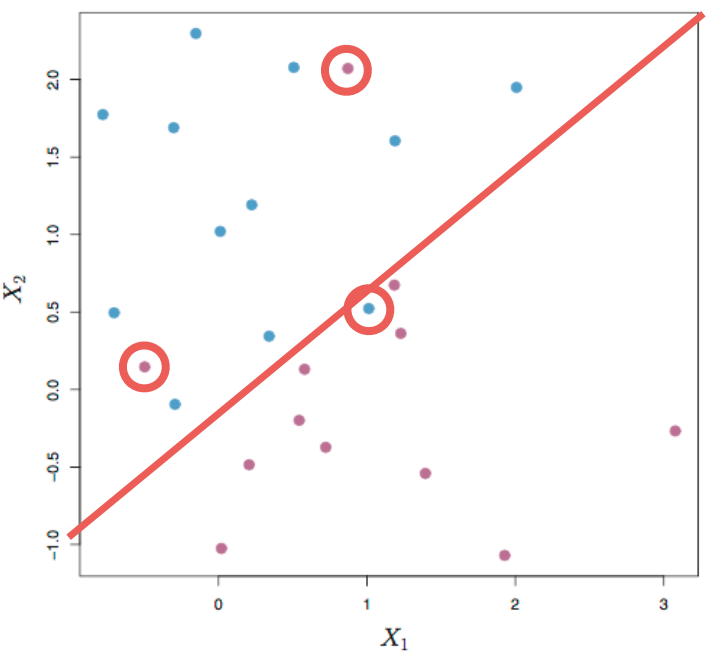
\includegraphics[width=\linewidth]{images/support-vector-machines/support-vector-machines-11.png}
  \end{column}
\end{columns}
\end{frame}


\begin{frame}{Support Vector Classifier}
\begin{columns}
  \begin{column}{0.5\textwidth}
    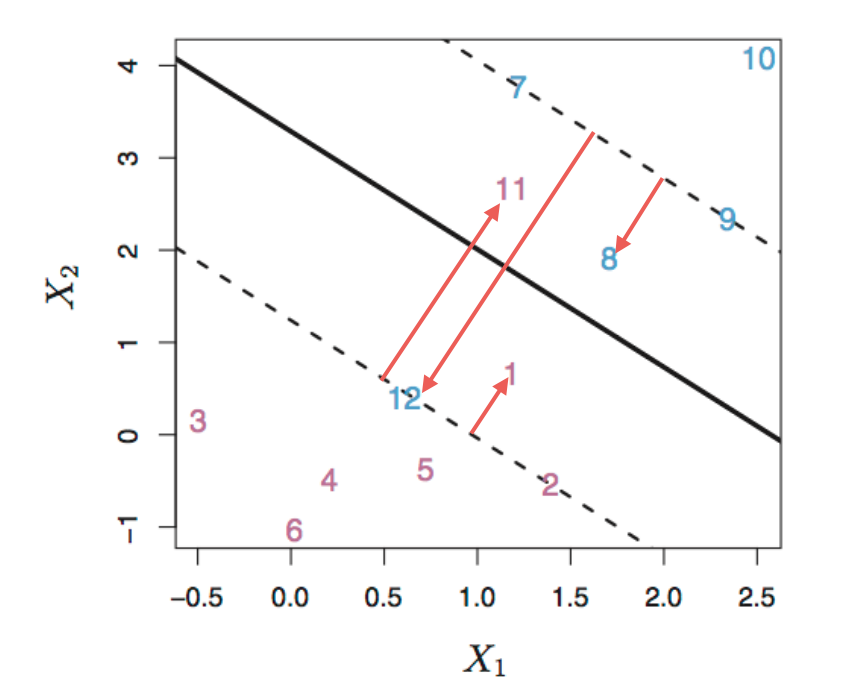
\includegraphics[width=\linewidth]{images/support-vector-machines/support-vector-machines-12.png}
  \end{column}
  \begin{column}{0.5\textwidth}
    \begin{itemize}
      \item Some points are allowed to violate the margin.
    \end{itemize}
  \end{column}
\end{columns}
\end{frame}


\begin{frame}{Support Vector Classifier}
\begin{columns}
  \begin{column}{0.5\textwidth}
    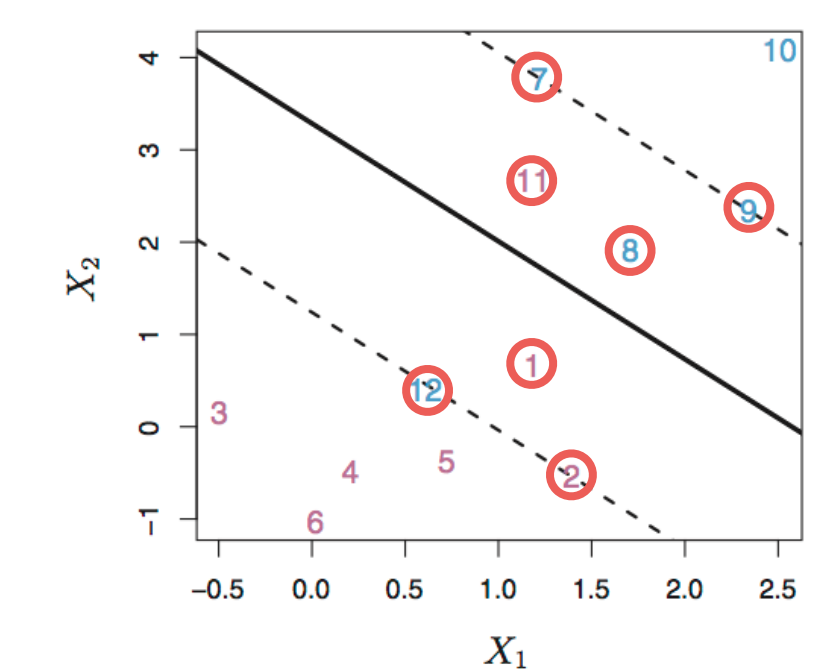
\includegraphics[width=\linewidth]{images/support-vector-machines/support-vector-machines-13.png}
  \end{column}
  \begin{column}{0.5\textwidth}
    \begin{itemize}
      \item Support vector classifiers also have support vectors.
      \item They are points lying directly on the margin, or on the wrong side of the margin for their class.
      \item These observations affect the hyperplane.
    \end{itemize}
  \end{column}
\end{columns}
\end{frame}



\begin{frame}{Finding Support Vector Classifier}
    \begin{itemsize}
        \item To find the support vector classifier hyperplane, solve:
    \end{itemsize}

    \[
    \max_{\beta_0, \ldots, \beta_p, \epsilon_1, \ldots, \epsilon_n} M
    \]

    \[
    \text{subject to } \sum_{j=0}^{p} \beta_j^2 = 1
    \]

    \[
    y^{(i)} \left( \beta_0 + \beta_1 x_1^{(i)} + \ldots + \beta_p x_p^{(i)} \right) \geq M (1 - \epsilon_i), \quad \forall i
    \]

    \[
    \sum_{i=1}^{n} \epsilon_i \leq C, \quad \epsilon_i \geq 0, \quad \forall i
    \]
\end{frame}


\begin{frame}{Support Vector Classifier}
    \begin{itemize}
        \item Slack variables $\epsilon_i$ allow for violations of the margin.
        \begin{itemize}
            \item $\epsilon_i = 0$: training point is on correct side of margin
            \item $\epsilon_i > 0$: training point violates the margin
            \item $\epsilon_i > 1$: training point is misclassified (wrong side of hyperplane)
        \end{itemize}
        \item Penalty parameter $C$ is the total ``budget'' for violations.
        \begin{itemize}
            \item Allows at most $C$ misclassifications on training set.
        \end{itemize}
    \end{itemize}
\end{frame}


\begin{frame}{How do we choose $C$?}
    \begin{itemize}
        \item As with many things we don’t know \textit{a priori} in machine learning, $C$ is a hyperparameter that we tune using cross-validation.
        \item Note that it must be non-negative.
        \item If $C = 0$, we recover the maximal margin classifier (if one exists).
        \item As $C$ goes from small to large, there is a bias-variance tradeoff.
    \end{itemize}
\end{frame}

\begin{frame}{Bias, Variance and $C$}
    \begin{columns}
        \begin{column}{0.45\textwidth}
            \begin{itemize}
                \item \textbf{Large $C$}
                \begin{itemize}
                    \item Large violation budget
                    \item Large margin
                    \item Many support vectors
                \end{itemize}
                \vspace{0.5cm}
                \item \textbf{Small $C$}
                \begin{itemize}
                    \item Small violation budget
                    \item Small margin
                    \item Few support vectors
                \end{itemize}
            \end{itemize}
        \end{column}
        \begin{column}{0.55\textwidth}
            \centering
            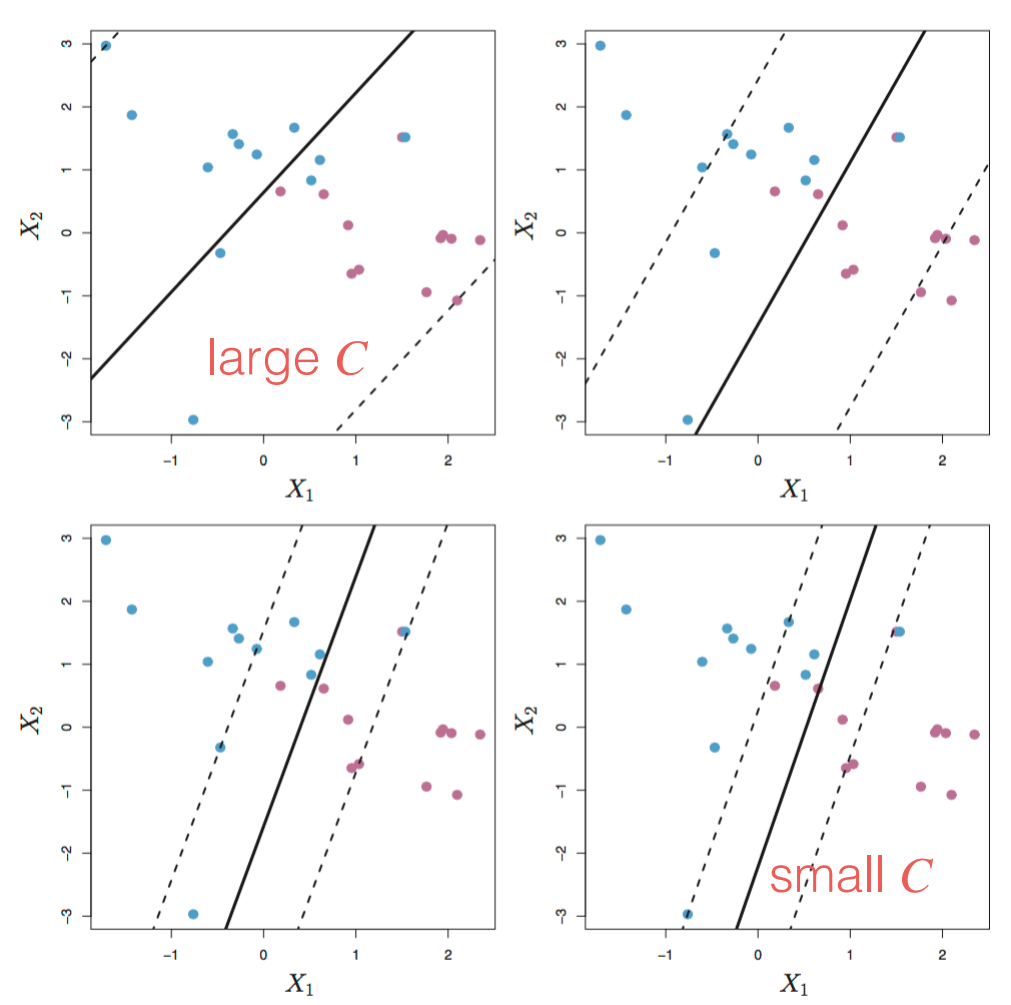
\includegraphics[width=\textwidth]{images/support-vector-machines/support-vector-machines-14.png}
        \end{column}
    \end{columns}
\end{frame}


\begin{frame}{Bias, Variance and $C$}
    \begin{columns}
        \begin{column}{0.45\textwidth}
            \begin{itemize}
                \item \textbf{Large $C$}
                \begin{itemize}
                    \item High bias
                    \item Low variance
                \end{itemize}
                \vspace{0.5cm}
                \item \textbf{Small $C$}
                \begin{itemize}
                    \item Low bias
                    \item High variance
                \end{itemize}
            \end{itemize}
        \end{column}
        \begin{column}{0.55\textwidth}
            \centering
            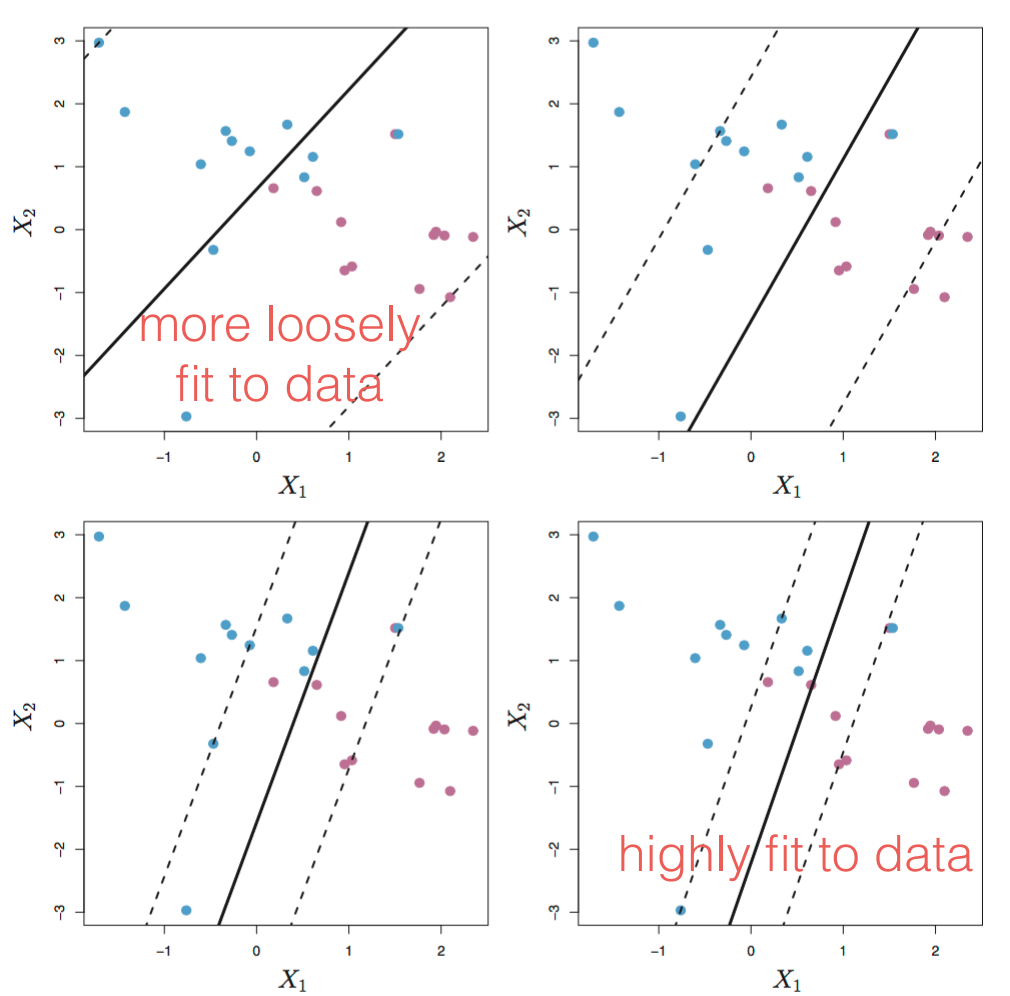
\includegraphics[width=\textwidth]{images/support-vector-machines/support-vector-machines-15.png}
        \end{column}
    \end{columns}
\end{frame}


\begin{frame}{Support Vector Classifier}
    \centering
    \textit{We are still using a \textbf{linear} decision boundary.}    
    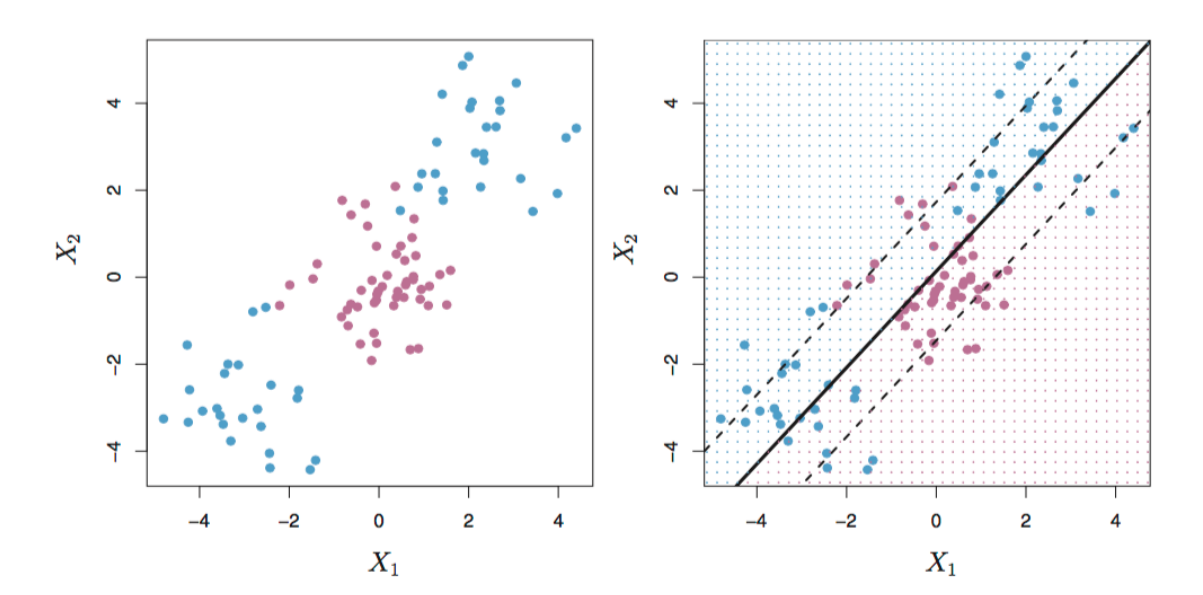
\includegraphics[width=0.9\textwidth]{images/support-vector-machines/support-vector-machines-16.png}
\end{frame}


\begin{frame}{Expanding Feature Space}
    \begin{columns}
        \begin{column}{0.55\textwidth}
            \small
            Some datasets are not linearly separable, but they \textit{become} linearly separable when transformed into a \textit{higher} dimensional space.

            \vspace{0.5cm}
            \textit{(Note: Yes, higher dimension also increases chance of overfitting. But in some cases the tradeoff is worthwhile.)}
        \end{column}
        \begin{column}{0.45\textwidth}
            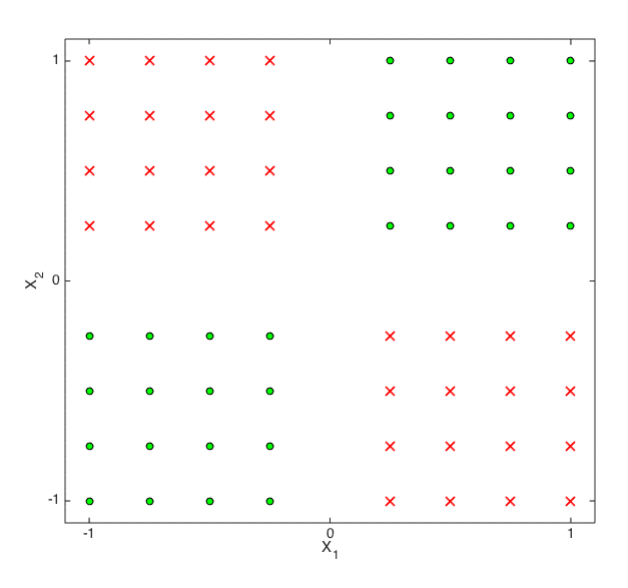
\includegraphics[width=\textwidth]{images/support-vector-machines/support-vector-machines-17.png}
        \end{column}
    \end{columns}
\end{frame}


\begin{frame}{Expanding Feature Space}
    \centering
    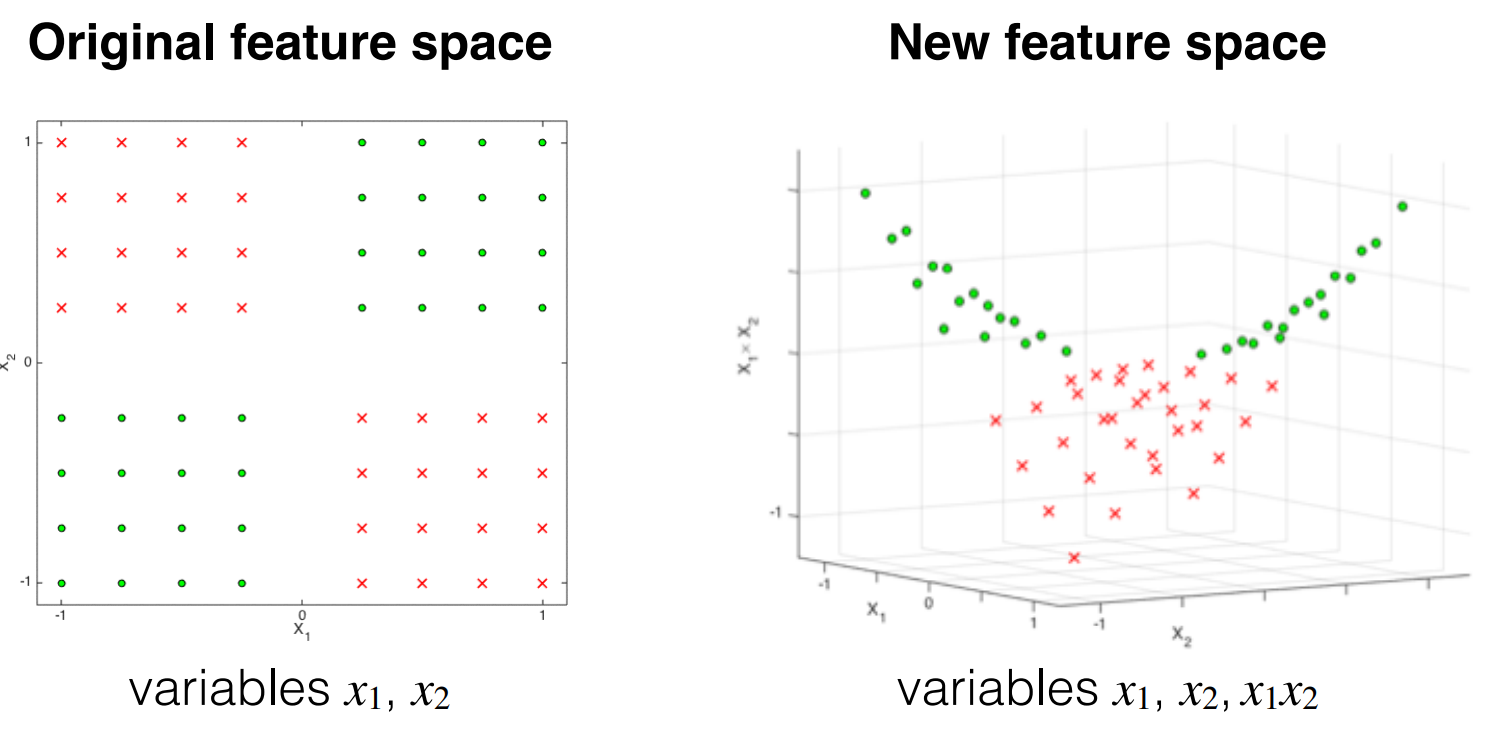
\includegraphics[width=\textwidth]{images/support-vector-machines/support-vector-machines-18.png}
\end{frame}


\begin{frame}{Expanding Feature Space}
    \begin{itemize}
        \item In linear regression, we created new features to capture non-linearity of data.
        \item For example:
        \[
        Y = \beta_0 + \beta_1 X_1 + \beta_2 X_1^2 + \epsilon
        \]
        \item We can apply the same technique to support vector classifiers.
    \end{itemize}
\end{frame}

\begin{frame}{Expanding Feature Space}
    \begin{itemize}
        \item Suppose our original data has $p$ features.
    \end{itemize}

    \[
    \vec{X} = (X_1, X_2, \ldots, X_p)
    \]

    \begin{itemize}
        \item We can expand the feature space to include e.g. $2p$ features.
    \end{itemize}

    \[
    \vec{X} = (X_1, X_1^2, X_2, X_2^2, \ldots, X_p, X_p^2)
    \]

    \[
    = (\tilde{X}_1, \tilde{X}_2, \tilde{X}_3, \tilde{X}_4, \ldots, \tilde{X}_{2p-1}, \tilde{X}_{2p})
    \]
\end{frame}

\begin{frame}{Expanding Feature Space}
    \begin{itemize}
        \item Support vector classifier will find a hyperplane in $2p$ dimensions:
    \end{itemize}

    \[
    \beta_0 + \beta_1 \tilde{X}_1 + \beta_2 \tilde{X}_2 + \cdots + \beta_{2p-1} \tilde{X}_{2p-1} + \beta_{2p} \tilde{X}_{2p} = 0
    \]

    \begin{itemize}
        \item Hyperplane will be non-linear in \textit{original} feature space. In this case, it is an ellipse:
    \end{itemize}

    \[
    \beta_0 + \beta_1 X_1 + \beta_2 X_1^2 + \cdots + \beta_{2p-1} X_p + \beta_{2p} X_p^2 = 0
    \]
\end{frame}


\begin{frame}{Non-linear Decision Boundary}
    \centering
    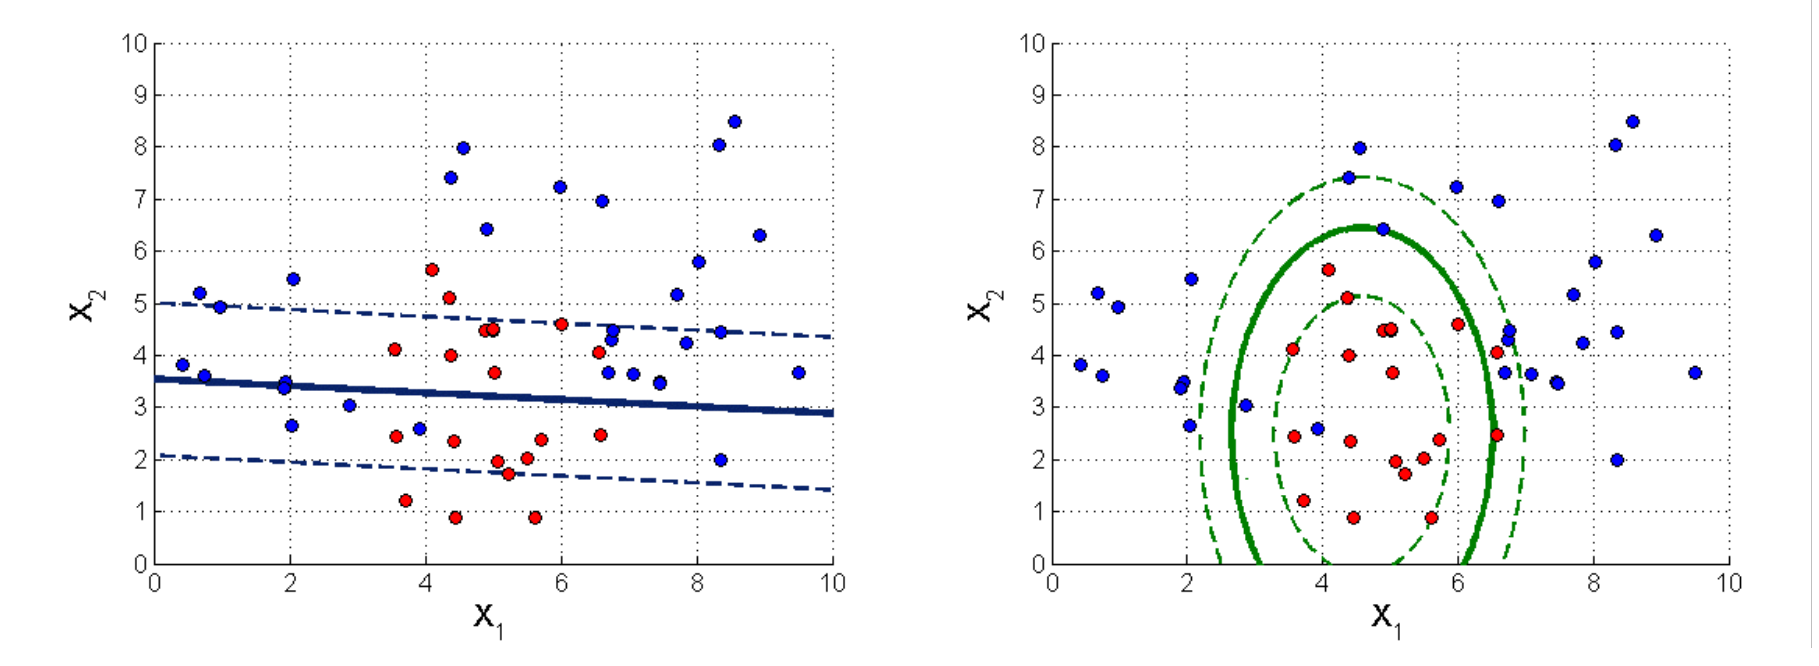
\includegraphics[width=\textwidth]{images/support-vector-machines/support-vector-machines-19.png}
\end{frame}



\begin{frame}{Expanding Feature Space}
    \begin{columns}
        \begin{column}{0.5\textwidth}
            \begin{itemize}
                \item Can imagine adding higher-order polynomial terms, quotients, and more to expand feature set.
                \item Large number of features becomes computationally challenging.
                \item We need an efficient way to work with large number of features.
            \end{itemize}
        \end{column}
        \begin{column}{0.5\textwidth}
            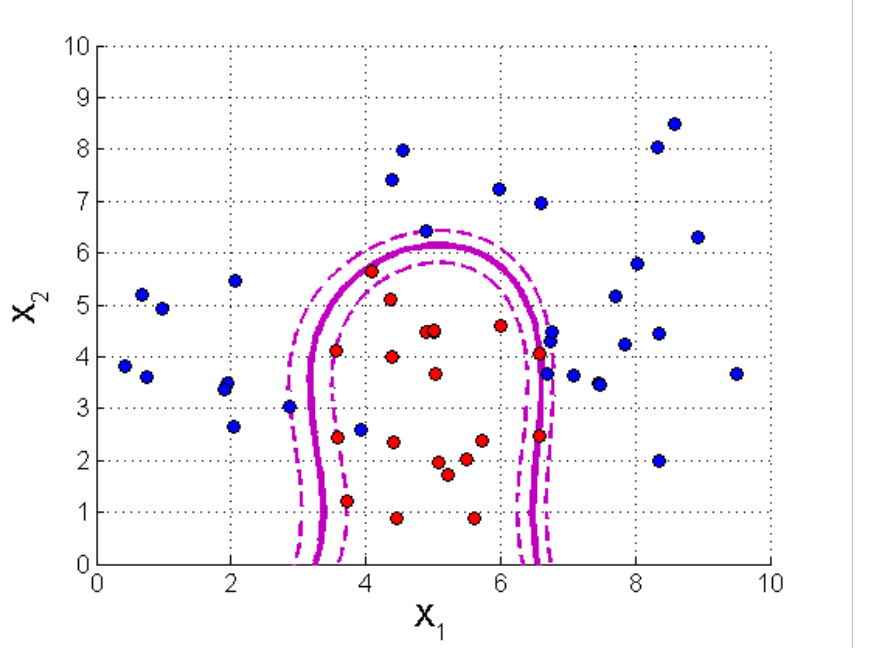
\includegraphics[width=\textwidth]{images/support-vector-machines/support-vector-machines-20.png}
        \end{column}
    \end{columns}
\end{frame}


